\begin{figure*}[t]
    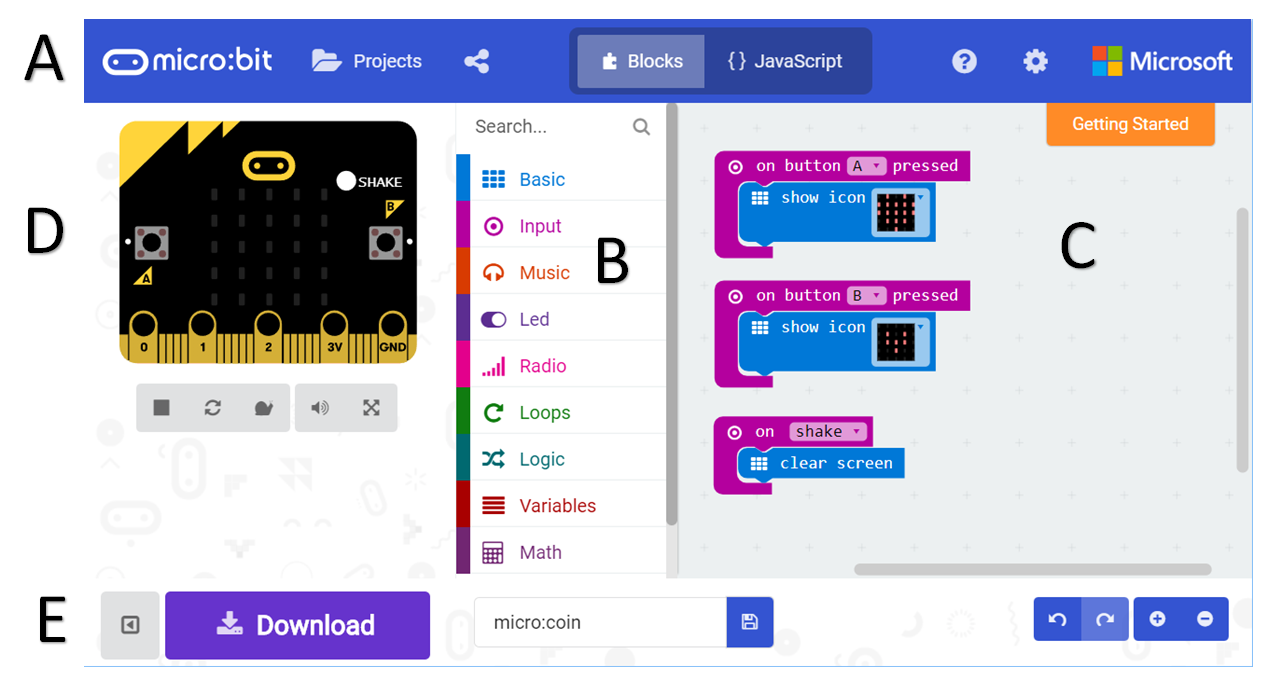
\includegraphics[width=6in]{images/webApp.png}
    \caption{\label{fig:snapshot}MakeCode web app for the micro:bit (\url{http://makecode.microbit.org}).}
  \end{figure*}

\section{The BBC micro:bit}
\label{sec:microbit}
% Talk about the motivations, make people care, provide concrete deliverables

The goals for the BBC micro:bit project were:
\begin{itemize}
    \item[B1] to provide a simple creative experience for physical computing, wearable and Internet of Things (IoT) projects;
    \item[B2] to supply a device that can continue to provide learning opportunities as the user's expertise grows.
    \item[B3] to give students an exciting, engaging introduction to coding;
    \item[B4] to stimulate curiosity about how computing technologies can be utilized to solve problems that students identify.
\end{itemize}

It's important to reiterate the context: delivering a micro:bit to every one of 
approximately 3/4 million Year 7 (5th grade) students and teachers in the UK, as
well as 1/4 million micro:bit outside of the school setting. This was a very
broad breadth engagement touching every community in the UK.

In the remainder of this section, we describe the hardware and software
of the micro:bit, the project history, and the experience deploying
the micro:bit in the UK.

\subsection{The hardware}

Figure~\ref{fig:microbit} shows (a) the front and (b) the back of the
micro:bit, which measures 4cm x 5cm. The aesthetic of the micro:bit is designed to be engaging from the start, with streaks of hair (upper left) and a friendly face (upper middle).
The micro:bit board hosts a variety of sensors (temperature, accelerometer, magnetometer,
light level), a 5x5 LED matrix, two user-defined buttons, as well as Bluetooth
Low Energy (BLE) communications.\footnote{The micro:bit has a whopping
16kB of RAM and 256kB of Flash memory, compared to the Uno's 2kB of
RAM and 32kB of Flash}. More importantly, the device embraces these sensors in its design bringing them to the fore, so to expose its users to the future: a world of embedded, Internet enabled devices.

In contrast to the Uno which has no built-in sensors, the micro:bit
allows many projects to be completed with no additional hardware or wiring.
The holes on micro:bit's edge connector allows additional external sensors 
and actuators to be connected via crocodile clips or banana plugs.
The micro:bit's BLE capabilities introduces networking to the
picture, and enables streaming of data and command/control operations among the micro:bit,
smartphones, laptops, as well as other micro:bits.
As with Arduino, an ecosystem of micro:bit shields
(hardware peripherals) that accommodate the micro:bit's edge
connector expands its capabilities (\url{http://microbit.org/resellers/}).

The micro:bit appears as a USB pen drive when plugged into a host computer;
a compiled program can be transferred to the micro:bit by a simple file copy
operation (flashed). The micro:bit then can be embedded in projects
where it runs on battery power.

The unique combination of features supplied by the micro:bit enables a creative,
extensive experience for physical computing (B1, B2). 
{\bf [TODO: make sure to note the novel contributions of the project, for those
readers with research hats on...]}

\subsection{The software}

The design of the micro:bit coding tools also was oriented towards a
simple starting experience with room for progression (B3, B4). Based on in-school trials with a micro:bit prototype, the BBC focused on delivering a web app
based on the popular Blockly framework~\cite{Blocky2015} to permit students to
create scripts via drag-and-drop operations in a web browser, and see
the execution of their scripts via a simulator; text-based coding via scripting languages also
was identified as an important feature. As the micro:bit would be incorporated
into standalone projects, it also was essential for the user's program to be stored on the device for future untethered execution via battery power.

%final design put the entire toolchain in web app, without need to invoke C/C++ compiler to
%compile the user's program; ARM DAPlink solution makes micro:bit appear as USB pen drive
%on all operating systems; MicroPython provided second programming solution with entire toolchain
%on the micro:bit!!]

% less techy here

The solution delivered by the BBC's partners evolved from the initial
design to include support for Blockly, JavaScript and Python, all
via web apps.
Figure~\ref{fig:snapshot} shows a screen snapshot of the MakeCode web app
for the micro:bit,
which supports programming via both Blocky and JavaScript.
The web app has five main sections: (A) menu bar with access to projects
and examples, and switching between Blockly and JavaScript editors; (B)
Blockly toolbox of micro:bit API categories; (C) Blockly programming
canvas with a simple reactive program; (D) micro:bit simulator for execution
of the user's program in browser; (E) download button, which invokes the in-browser
compiler/linker to produce a binary executable.

The Python solution for the micro:bit is based on MicroPython (\url{http://micropython.org})
an implementation of Python 3.0 for microcontrollers. It includes
a full Python compiler and runtime that runs on the micro:bit and
supports a read-eval-print loop (REPL) to execute commands sent via
a terminal, as well as to import and run scripts from the Python web app for
the micro:bit (\url{http://python.microbit.org}).

\subsection{Content, training and events}

Great hardware and software do not a full solution make. Therefore,
the BBC micro:bit project also called for partners to develop content,
to ``train the trainers'' (educators) around the micro:bit computing
system, and provide hands-on events outside of the school setting to
generate interest in the micro:bit.

{\bf [TODO: more about what was developed by the partners ]}

\subsection{End-to-end experience}

We run through a simple coding example for the micro:bit, as shown
in Figure~\ref{fig:snapshot}(C). The event-based program shown there
in the Blockly editor displays a large heart when the
A button is pressed, displays a small heart when button B is pressed,
and clears the display when the user shakes the micro:bit (shake
detection is implemented using the accelerometer). The interactive
micro:bit simulator
(Figure~\ref{fig:snapshot}(D)) allows the user to test that
the program works as expected. In the simulator, the
shake event is fired using a virtual button (white circle labelled
``SHAKE'').

To generate a binary executable for the micro:bit, the user
simply presses the ``Download'' button (Figure~\ref{fig:snapshot}(E)),
which invokes an in-browser compiler tool chain that translates
the Blockly program to JavaScript and then to machine code, linking
the user's compiled code against a pre-compiled
C++ runtime. This means that no C++ compiler is required for
compiling the user's program.

{\bf [what about copying file and the fact that this works across many
platforms, including ChromeBooks! ]}
% \item ARM's DAPlink firmware makes the micro:bit appear as USB pen drive
% on most operating systems, enabling a simple file copy operation to
% install a user's program on the micro:bit (no device drivers needed).


% \begin{itemize}
% \item
% \item an efficient C++ runtime for the micro:bit created by Lancaster
% University;
% \item a web app
% with Blockly and JavaScript editors, micro:bit simulator,
% and a compiler to machine code (linked against a pre-compiled
% C++ runtime image, so no C++ compiler is needed for user code);
% \item a Python compiler and read-eval-print loop (REPL) that resides
% {\em on the micro:bit} (via \url{https://micropython.org/}),
% supported by a simple web app (\url{http://python.microbit.org}) and
% an installable application (\url{https://codewith.mu/});

% \end{itemize}

%- A lot of lessons learned from delivering end-to-end experience in UK and other countries
%   - hardware (unique design, as already mentioned)
%   - firmware:  high-level C/C++ runtime and ARM's DAPlink
%   - web-based IDE: no C/C++ compiler needed to compile user code
%   - content
%   - training
% In country partnerships

% main points
% - mass participation
% - country readiness (or perhaps willingness)

% compared to Arduino
% https://twitter.com/adamwwolf/status/1019070808038072320

% success of micro:bit due to
% - Low-cost, simplicity
% - Partnerships (hardware, software, content, training)
% - Open Source of software (CODAL, MakeCode, ...)
% - Hardware Reference design

% - why is it interesting?
%   - edge/physical/IoT computing
%   - build off of Scratch/Blockly, but untethered (via in-browser compiler)
%   - transition to JavaScript and Python

% - BBC rollout in UK
% - Global reach
%    - BBC rollout mirrored in other countries
%    - Communities
%      - Sri Lanka user group: http://microbitslug.org/
%      - UK libraries (loan program)
%    - third party editors


\subsection{Project history and open sourcing}


Previous papers with micro:bit history:

\begin{itemize}
    \item \cite{rogers2017bbc} - A brief history of micro:bit, unclear to me if we should include or duplicate.
    \item \cite{sentance2017creating} - Sue Sentance paper on kids creating stuff with micro:bit
    \item \cite{knowles2018children} - Lancaster paper on what children want to create using the micro:bit -- inspirational?
\end{itemize}

As mentioned in the Introduction, the motivation for the BBC micro:bit project
stemmed from the BBC's previous history with computing education and the BBC Micro
project, the desire to address the growing digital divide in the UK~\cite{XYZ},
as well as the UK government's mandate to teach computer science at the K-12 grade levels.

{\bf [Why did the BBC choose physical computing? Really need Howard Baker's input on this]}

{\bf [2014 BBC reference implementation: \url{https://github.com/bbcmicrobit/prototype}
by Michael Sparks ]}

{\bf [user trials with the prototype - how did BBC determine Year 7 was the right year?] }

In December 2014, the BBC issued an Request for Participation
for ``Delivery of a hands-on learning experience for the Make it Digital season'',
which was the micro:bit project.
Twenty-nine partners were invited to contribute hardware, software, services,
teaching materials, packing/distribution, logistics, events and funding.
Work on the project commenced in February 2015, with delivery of
a web site/app in September 2015 (which was critical
for training teachers) and delivery of the micro:bits in the second
half of the 2015-2016 school year.

The BBC micro:bit project partners agreed to open source all assets, both
hardware and software. The main entry points are:
\begin{itemize}
\item \url{https://github.com/bbcmicrobit} for MicroPython, hardware, and prototype;
\item \url{https://github.com/microsoft/pxt} for Microsoft MakeCode;~\footnote{
MakeCode superceded the TouchDevelop for micro:bit web app~\cite{ball2016microsoft}, also developed by Microsoft.    
}
\item \url{https://github.com/lancaster-university/microbit-dal} for the micro:bit
C++ runtime.
\end{itemize}


\subsection{UK rollout}

{\bf [ give some detail about how it went and reference studies of Sue Sentance and
UCL...]}

% maybe not, unsure... EE1 == educational expert one (i.e. clare riley). We would need to add two sentences on methodology.
Teacher education and training plays an important role in the uptake of technology in the classroom. As part of the micro:bit project, EE1 directed the curriculum-oriented resource curation and the coordination of training sessions. These were run with CAS~\cite{crick2011computing} `master' teachers and operators of extra curricular clubs like UKYouth, Code Club, and CoderDojo. Recipients of the training would be responsible for continuing dissemination at schools and clubs in their vicinity creating a ``cascade effect of teacher training which was really powerful''.

EE1 described the main challenge of this aspect to the micro:bit project was ``trying to get everybody capable to do it and enthusiastic'', she described it as hard work because the teachers who lack a strong background in computing were ``a bit nervous about all of this, and they are alarmed at the prospect of having to teach computing''. She engaged with a wider group of organisations (UKYouth, Code Clubs, CoderDojos) that are passionate about technology and computing who have the experience and the background, and through training both, one could provide support for the other, offering breadth and support---not only for the young people, but for the teachers as well.

Training consisted of a familiarisation session with the device and code editors, guiding teachers through lesson plans and discussing how the lesson plan met the criteria of the UK curriculum; they were encouraged to play, tweet and blog for the remaining time. EE1 noted that the response from her audience to the training sessions was incredible, with a general response of ``100\% wow, let's get going''. She related a story describing the experience of one teacher who before commencing training believed that this was ``another rubbish project from people who'd spent too much money the wrong way'', but after engaging with the micro:bit loved it. She pointedly explained that she expected this reaction, as the people who attended the sessions weren't techno-phobes, while a much harder challenge was to reach those who were.

From using the CAS network of teachers, EE1 learned that less confident teachers were not comfortable with the single-lesson plan approach of teaching the curriculum. She explained that they ``wanted a 6 or 8 week block of stuff, which said `this is the scheme of work which will deliver these outcomes from the national curriculum''', rather than the individual lessons---they wanted more scaffolding.

Overall, from our interviews, we saw that the cascading of teacher training, combined with the engagement of enthusiastic technologists, alongside structured curriculum-aligned resources are clear contributors to the uptake of the micro:bit.


